\documentclass[]{article}
\usepackage{caption,subcaption,graphicx,float,url,amsmath,amssymb,tocloft}
\usepackage[hidelinks]{hyperref}
\usepackage[toc,acronym,nonumberlist]{glossaries}
\setacronymstyle{long-short}
\usepackage{glossaries-extra}
\graphicspath{{figs/}} 
\setlength{\cftsubsecindent}{0em}
\setlength{\cftsecnumwidth}{3em}
\setlength{\cftsubsecnumwidth}{3em}

%opening
\title{
	Notes from Origins of Life\\
	Week 5: Evolution}
\author{Simon Crase}

\makeglossaries

\loadglsentries{glossary-entries}

\renewcommand{\thesection}{5.\arabic{section}}
\renewcommand{\glstextformat}[1]{\textbf{\em #1}}
\newcommand{\E}{\mathrm{E}}
\newcommand{\Var}{\mathrm{Var}}
\newcommand{\Cov}{\mathrm{Cov}} 
\newcommand\numberthis{\addtocounter{equation}{1}\tag{\theequation}}

\begin{document}

\maketitle

\begin{abstract}
   These are my notes from the $5^{th}$ Week of the Santa Fe Institute Origins of Life Course\cite{sfi2019}. The course aims to push the field of Origins of Life research forward by bringing new and synthetic thinking to the question of how life emerged from an abiotic world.\\
   The content and images contained herein are the intellectual property of the Santa Fe Institute, with the exception of any errors in transcription, which are my own.
   These notes are distributed in the hope that they will be useful,
   but without any warranty, and without even the implied warranty of
   merchantability or fitness for a particular purpose. All feedback is welcome,
   but I don't necessarily undertake to do anything with it.
\end{abstract}

\setcounter{tocdepth}{2}
\tableofcontents
\listoffigures

\section{Introduction}

We discuss Selection, Phylogenetics, Macroscopic Regularities across all of life, how has life evolved in creating Complexity, and evolutionary processes in Artificial Life. 

\section{Origins of Eukaryotes}

Lecturer: David Baum

Cellular life began prokaryotic: metabolic and genetic systems enclosed in a single
boundary.

Eukaryotic cells evolved once; we don't have intermediate steps.

\begin{itemize}
	\item Many internal membrane-bound structures
	\begin{itemize}
		\item nucleus
		\item mitochondria
		\item endomembrane system)
	\end{itemize}
	\item A significant evolutionary event!
\end{itemize}

\begin{itemize}
	\item Cellular predators--Figure \ref{figs:Cellular:predators:symbiotic:hosts1}--the lions and tigers of the micro-biotic world!
	\item Symbiotic hosts--Figure \ref{figs:Cellular:predators:symbiotic:hosts2}-- the farmers of the micro-biotic world!
	\item Multicellularity
	\begin{itemize}
		\item why have only eukaryotes evolved multicellularity?
		\item Why have eukaryotes evolved it multiple times? The best known instances are animals, plants, and fungi, but there are others.
	\end{itemize}
\end{itemize}

\begin{figure}[H]
	\caption{Cellular predators, symbiotic hosts}
	\label{figs:Cellular:predators:symbiotic:hosts}
	\begin{subfigure}[b]{0.45\textwidth}
		\caption{ }
		\label{figs:Cellular:predators:symbiotic:hosts1}
		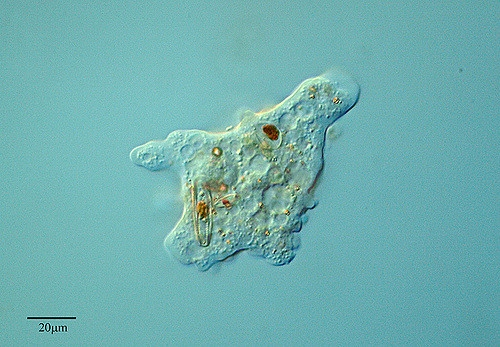
\includegraphics[width=\textwidth]{Eukaryotes1}
	\end{subfigure}
	\begin{subfigure}[b]{0.45\textwidth}
		\caption{ }
		\label{figs:Cellular:predators:symbiotic:hosts2}
		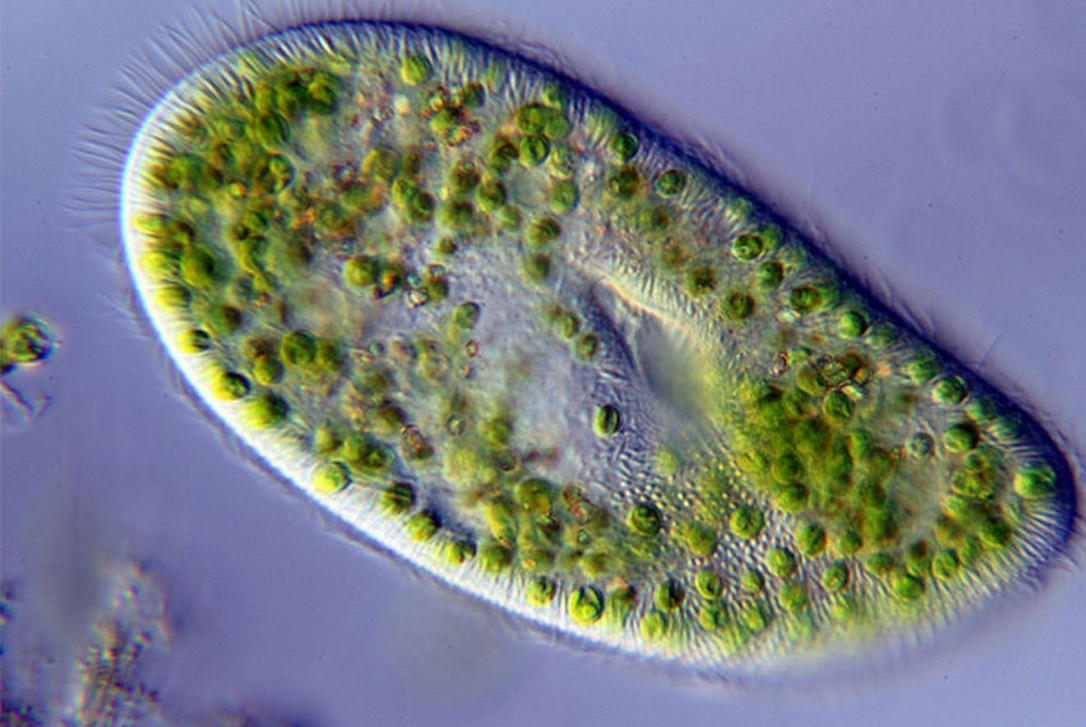
\includegraphics[width=\textwidth]{Eukaryotes2}
	\end{subfigure}
\end{figure}
Why eukaryotes? There are three ideas at present.

\begin{itemize}
	\item Mitochondria improve energetic efficiency, and allow energy use to be regulated more nimbly.\cite{lane2010energetics}.
	
	\item Flexible membranes allow phagocytosis and generation of internal vesicles. So eukaryotes can do things that prokaryotes can't, such as engulfing food prey--Figure \ref{fig:engulf}.
	
	\item Nucleus and \gls{gls:endomembrane} system allow for finer gene
	regulation--Figure \ref{fig:finer:gene:regulation}\cite{paez2016endocytosis}. 
	\begin{itemize}
		\item Multicellular organization requires communications between different cells, which express different genes and proteins.
		\item The extra layers of regulation that eukaryotes have may explain why they, and not prokaryotos, have evolved complex multicellular organisms. These layers deal with the genetic control by separating the transcription of a DNA sequence from the reading of the message--there are many steps where regulation can be imposed. 
		\item Additionally the \gls{gls:endomembrane} system can affect the secretion, degradation and recycling of proteins
	\end{itemize}
\end{itemize}

\begin{figure}[H]
	\caption{Flexible membranes allow phagocytosis and generation
		of internal vesicles}
	\label{fig:engulf}
	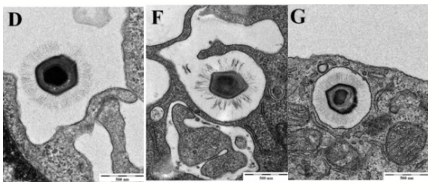
\includegraphics[width=0.9\textwidth]{Engulf}
\end{figure}


\begin{figure}[H]
	\caption{Nucleus and endomembrane system allow for finer gene
		regulation}\label{fig:finer:gene:regulation}
	\begin{subfigure}[b]{0.45\textwidth}
		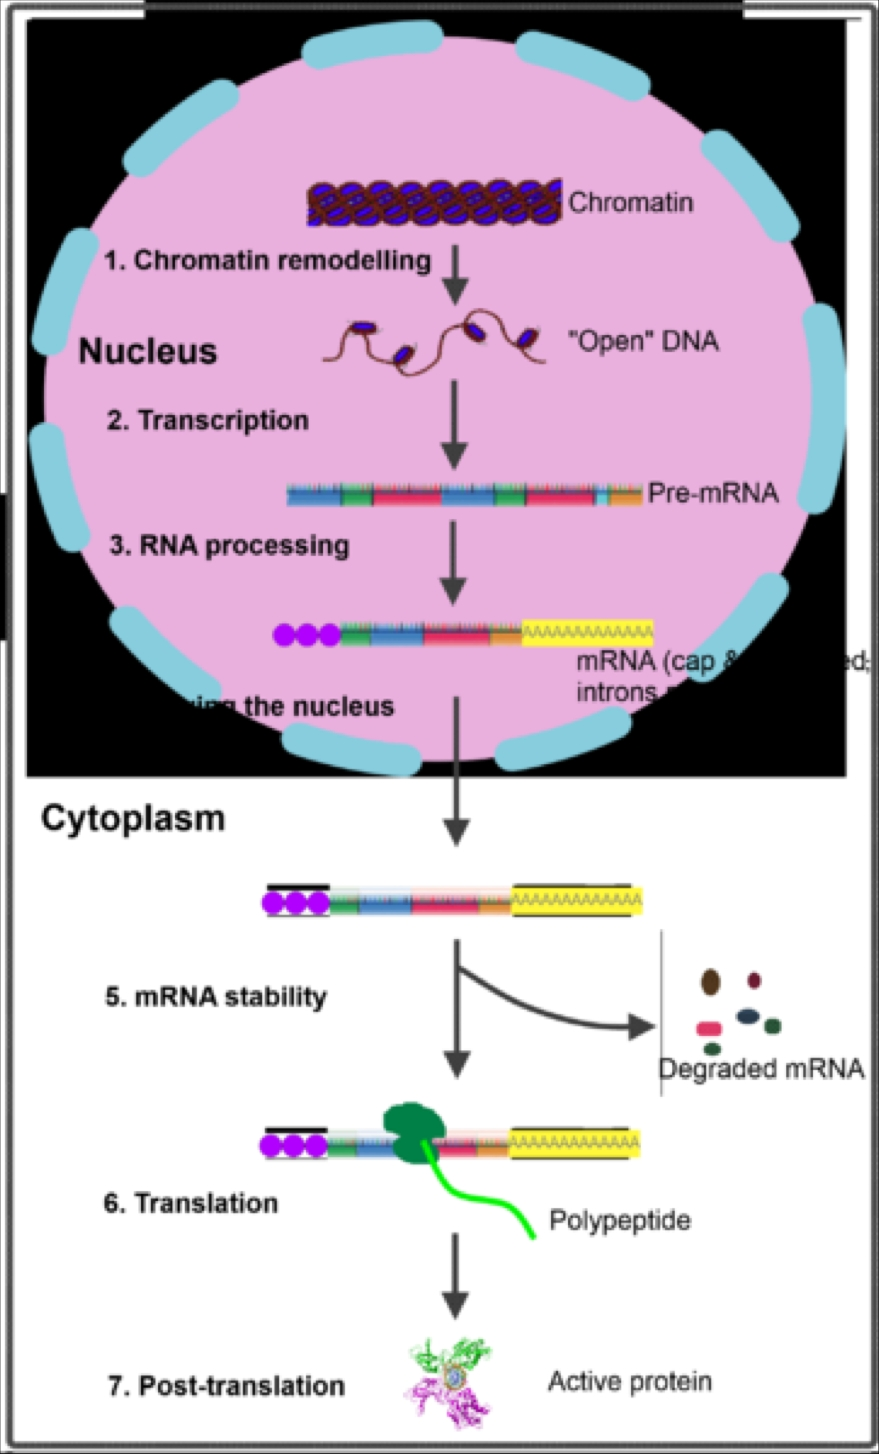
\includegraphics[width=\textwidth]{Regulation1}
	\end{subfigure}
	\begin{subfigure}[b]{0.45\textwidth}
	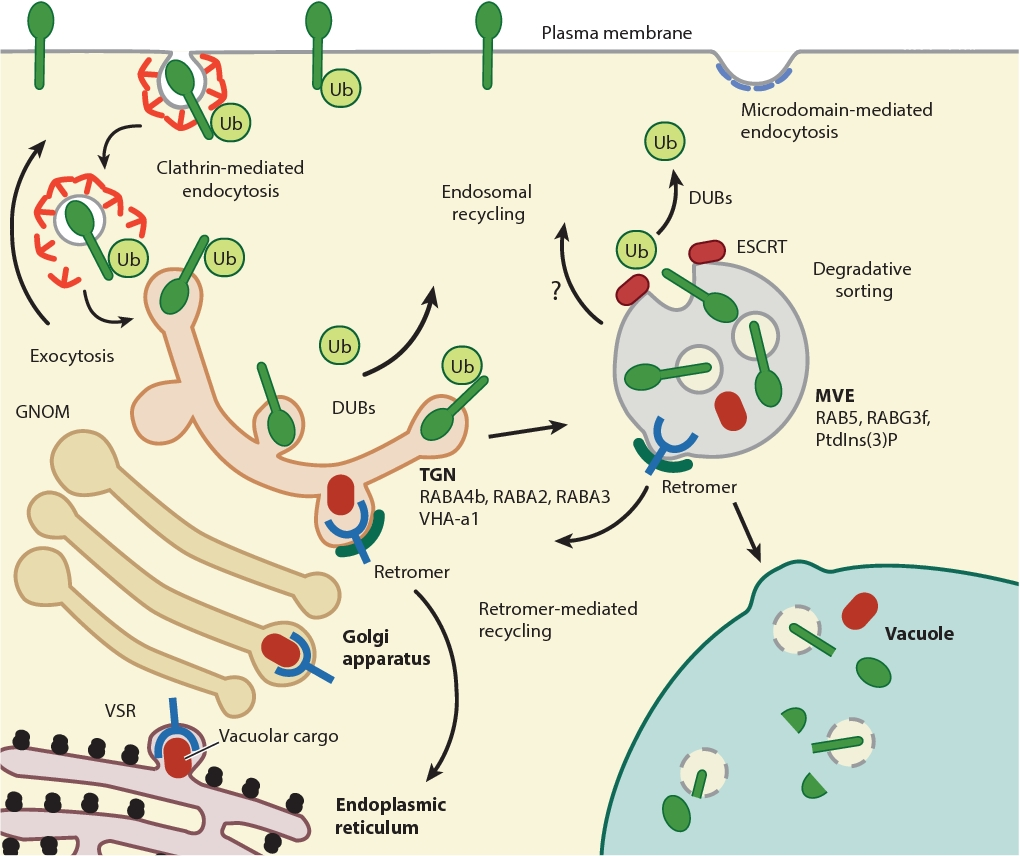
\includegraphics[width=\textwidth]{Regulation2}
	\end{subfigure}
\end{figure}
Easier to study than the
origin of life

\begin{itemize}
	\item We can use phylogenetic methods to infer the features of \gls{gls:LECA}--Figure \ref {fig:LECA}. We can study both ends of the \gls{gls:LECA} branch, since we have procaryotes; we cannot do this with \gls{gls:LUCA}.
	\begin{itemize}
		\item Mitochondria are endosymbiotic bacteria\cite{germot1996presence}
		\item Host was an archaeon\cite{spang2015complex}
		\item Can distinguish genes of archaeal or
		bacterial ancestry\cite{thiergart2012evolutionary}
	\end{itemize}
\end{itemize}

\begin{figure}[H]
	\caption{LECA}\label{fig:LECA}
	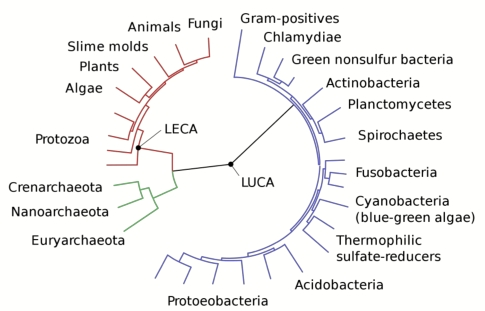
\includegraphics[width=0.9\textwidth]{LECA}
\end{figure}

\begin{figure}[H]
	\caption{Mitochondria are endosymbiotic bacteria}
	\label{fig:Mitochondria:are:endosymbiotic:bacteria}
	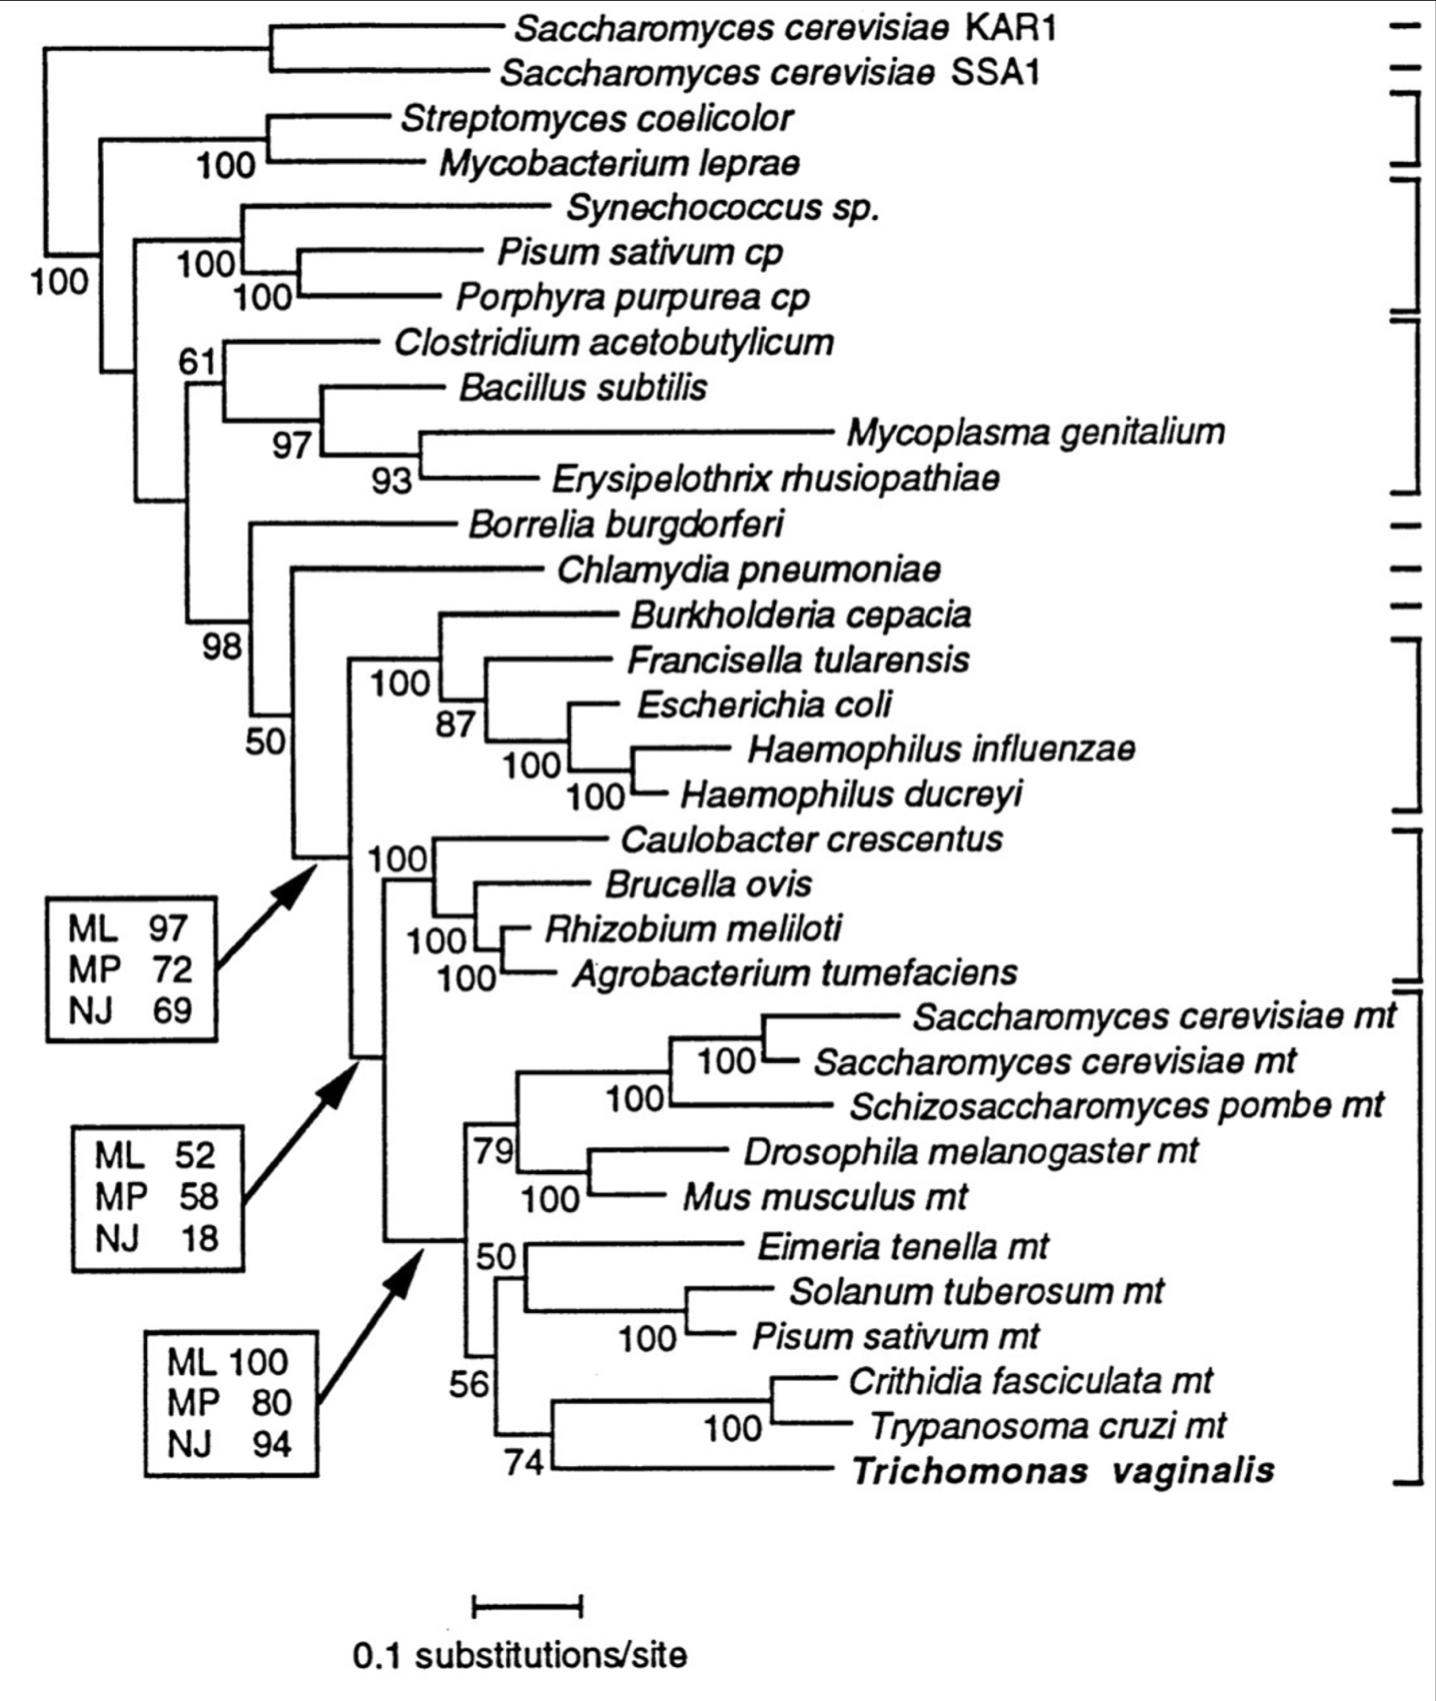
\includegraphics[width=0.9\textwidth]{MitochondriaEndosymbiotic}
\end{figure}

\begin{figure}[H]
	\caption{Host was an archaeon}
	\label{fig:host:archaeon}
	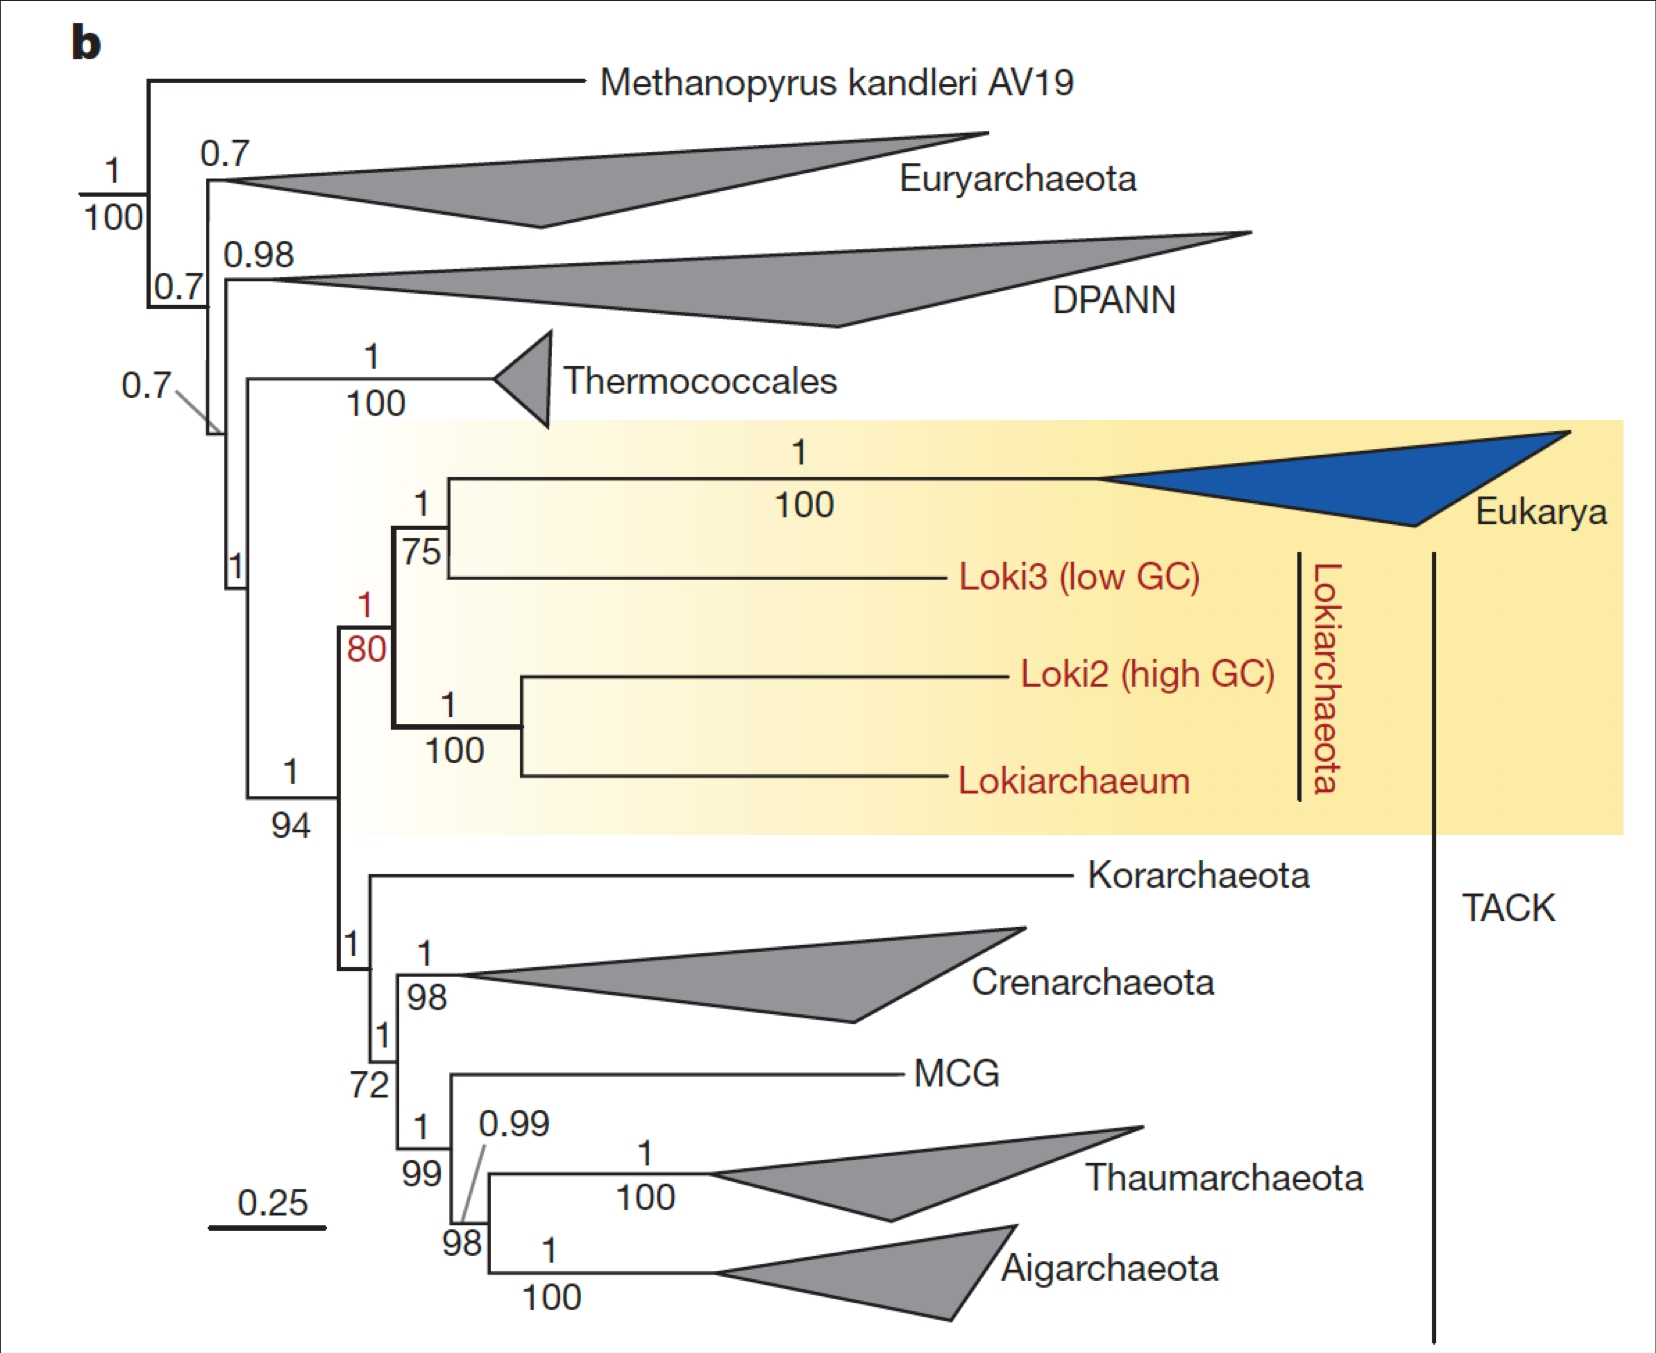
\includegraphics[width=0.9\textwidth]{HostArchaeon}
\end{figure}

\begin{figure}[H]
	\caption{Can distinguish genes of archaeal or bacterial ancestry}
	\label{fig:distinguish:genes:archaeal:bacterial}
	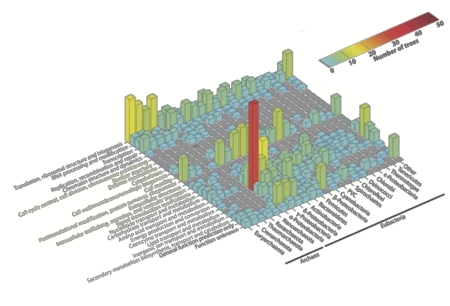
\includegraphics[width=0.9\textwidth]{thiergart2012}
\end{figure}

Mysteries remain
\begin{itemize}
	\item How did a bacterium get into an archaeon? There are two extremes in a range of theories.
	\begin{itemize}
		\item In the Outside-in Model, and archaean developed a membrane, Figure \ref{fig:outside:in1}, which became invaginated. It enveloped mitochondria in a mutualistic association--Figure \ref{fig:outside:in2}. Later it developed membranes to protect DNA from the activity (free oxygen) of the mitochondria--Figure \ref{fig:outside:in3}--until the nucleus was fully enclosed--Figure \ref{fig:outside:in4}.
		\item In the Inside-out Model--Figure \ref{fig:inside:out}--the cell becomes associated with arachaea, which are gradually walled in \cite{baum2014inside}.
	\end{itemize}
	\item How was a nucleus formed?
\end{itemize}

\begin{figure}[H]
	\caption{Outside-in Model}\label{fig:outside:in}
	\begin{subfigure}[b]{0.45\textwidth}
		\caption{ }\label{fig:outside:in1}
		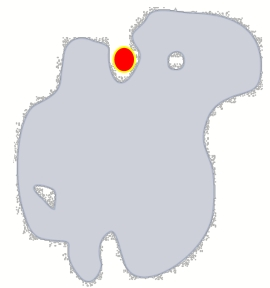
\includegraphics[width=\textwidth]{OutsideIn1}
	\end{subfigure}
	\begin{subfigure}[b]{0.45\textwidth}
		\caption{ }\label{fig:outside:in2}
		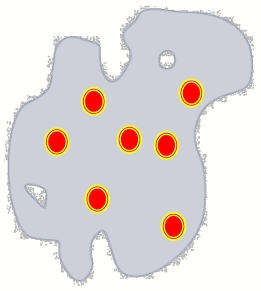
\includegraphics[width=\textwidth]{OutsideIn2}
	\end{subfigure}
	\begin{subfigure}[b]{0.45\textwidth}
		\caption{ }\label{fig:outside:in3}
		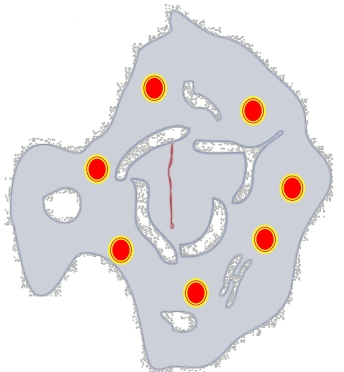
\includegraphics[width=\textwidth]{OutsideIn3}
	\end{subfigure}
	\begin{subfigure}[b]{0.45\textwidth}
		\caption{ }\label{fig:outside:in4}
		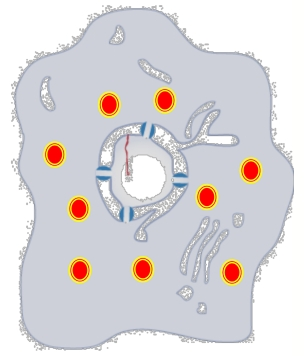
\includegraphics[width=\textwidth]{OutsideIn4}
	\end{subfigure}
\end{figure}

\begin{figure}[H]
	\caption{Inside-Out Model}\label{fig:inside:out}
	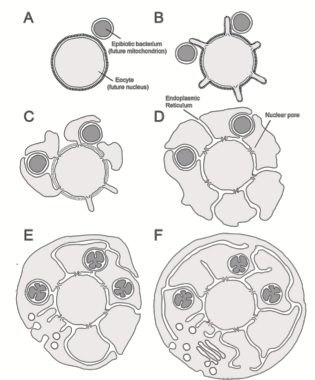
\includegraphics[width=0.9\textwidth]{InsideOut}
\end{figure}

But still easier to solve than the origin of life!
\begin{itemize}
	\item New genomic data keep emerging
	\item There is a possibility of finding intermediates
\end{itemize}

\cite{javaux2003recognizing},  

\section{\Gls{gls:phylogenetics}}


\subsection{Using Phylogenetics to Travel in Time}
Lecturer: Bet{\"u}l Ka{\c c}ar

A phylogenetic tree is an hypothesis, not an established fact. Key Points:
\begin{itemize}
	\item A phylogenetic tree demonstrates evolutionary
	relationships among genes, proteins or organisms.
	\item In a phylogenetic tree, two species are closely
	related if they have a more recent shared ancestor.
\end{itemize}

\begin{itemize}
	\item $\approx 1.2$ million eukaryotes catalogued
	\item $\approx 8.9$ million eukaryotes present on Earth
	\item $>99\%$ of species have gone extinct thus severally limiting our starting pool
\end{itemize}

Tree Thinking and phylogeny
\begin{itemize}
	\item The evolutionary history of a group is its phylogeny
	\begin{itemize}
		\item Since we can’t travel back in time to identify
		common ancestors relationships of existing
		species must be estimated or inferred from data
	\end{itemize}
	\item The branching pattern in a phylogenetic tree illustrates how organisms evolved from a list of common ancestors.
	\item The evolutionary history of extant organisms can
	be understood in terms of their shared inheritance
	\begin{itemize}
		\item which extant species evolved from the same ancestor?
		\item how were ancestral traits modified in different lineages?
	\end{itemize}
\end{itemize}

\begin{figure}[H]
	\caption{Often there are many ways to model relationships, but generally the simplest will be most accurate.}\label{PhylogenicTree}
	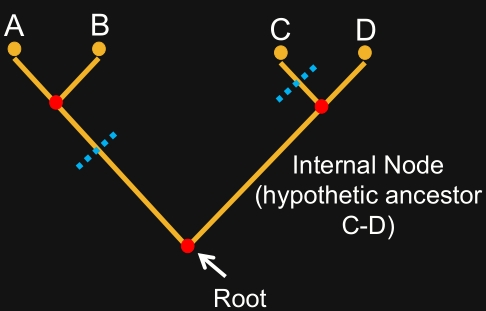
\includegraphics[width=0.9\textwidth]{PhylogenicTree}
\end{figure}

\begin{figure}[H]
	\caption{Molecular Phylogenetics Protocol}\label{fig:MolecularPhylogeneticsProtocol}
	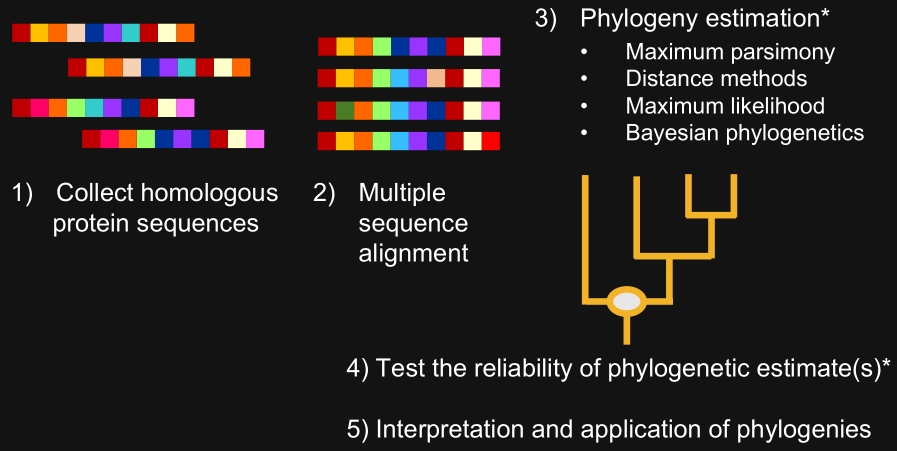
\includegraphics[width=0.9\textwidth]{MolecularPhylogeneticsProtocol}
\end{figure}
Some other applications of phylogenetics
\begin{itemize}
	\item Classification and taxonomy of genes, proteins and species
	\item Comparative analysis and character evolution
	\item Predicting protein structure and function
	\item Investigating the history and demography of populations
	\item Studying the emergence and spread of viral and bacterial pandemics
	\item Searching for useful traits in related groups
\end{itemize}

\begin{figure}[H]
	\caption{Phylogenetic Tree of Life--The big picture}
	\label{flg:the:big:picture}
	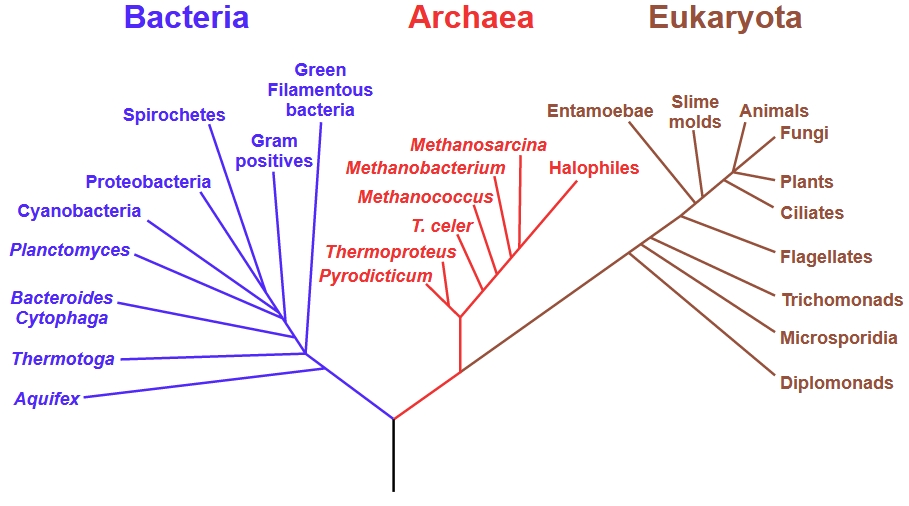
\includegraphics[width=0.9\textwidth]{TOL5}
\end{figure}

See \cite{hillis1996molecular}, \cite{zuckerkandl1965molecules}, \cite{williams2006assessing}, \cite{woese2002evolution}

\subsection{A Deeper Dive into Phylogenetics}

Lecturer: Andy Rominger
\begin{itemize}
	\item How to Infer a Phylogeny
	\item Why is the Deep Past so difficult to Infer?
\end{itemize}

\subsubsection{How to Infer a Phylogeny}
We are going to focus on step 3 of Figure \ref{fig:MolecularPhylogeneticsProtocol}, finding the evolutionary process leading to the data we have. We start with homologous sequences, and we want to infer the speciation, extinction, and passing genes on to daughter lineages.

We have transition rates, topology, and sequence data--Figures \ref{fig:InferringPhylogeny} \& \ref{fig:InferringPhylogeny1}, and we want to choose transition rates and a topology to \textit{maximize the likelihood}--Figures \ref{fig:InferringPhylogeny2}. 

\begin{figure}[H]
	\caption{Inferring a phylogeny}\label{fig:InferringPhylogeny}
	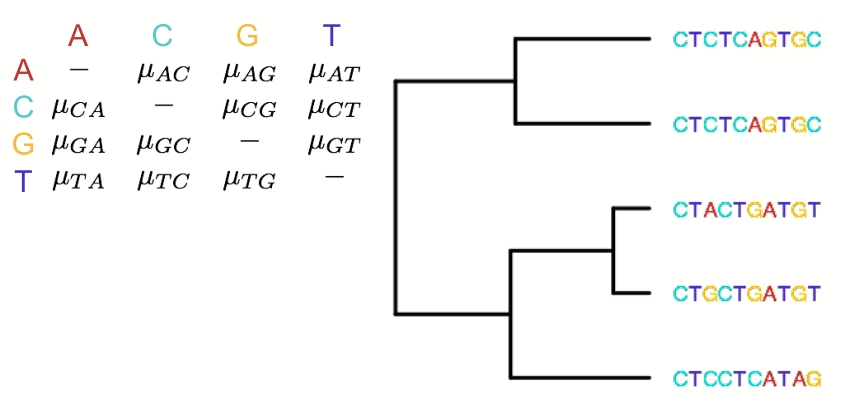
\includegraphics[width=0.9\textwidth]{InferringPhylogeny}
\end{figure}

\begin{figure}[H]
	\caption{Goal: find the process leading to the data}\label{fig:InferringPhylogeny1}
	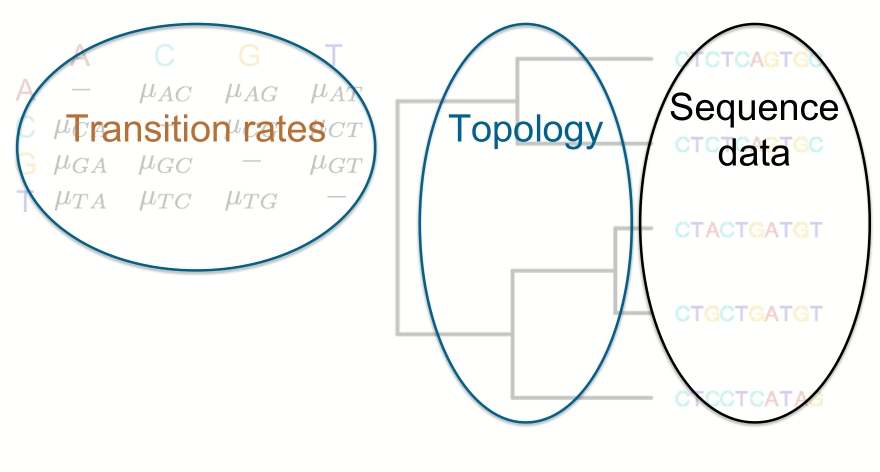
\includegraphics[width=0.9\textwidth]{InferringPhylogeny1}
\end{figure}

\begin{figure}[H]
	\caption{Maximize Likelihood}\label{fig:InferringPhylogeny2}
	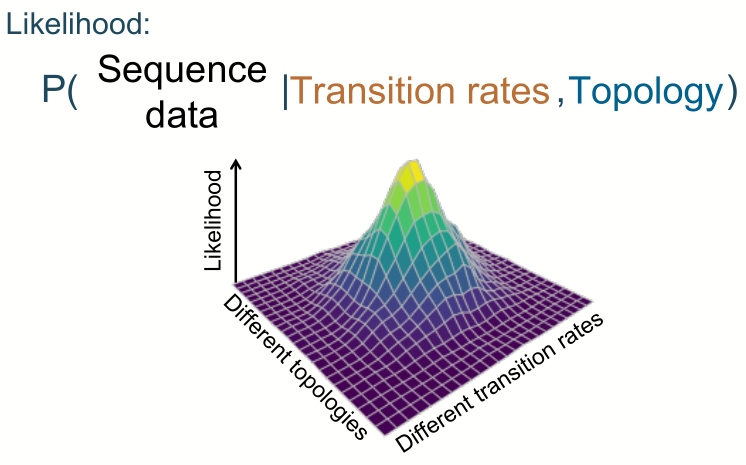
\includegraphics[width=0.9\textwidth]{InferringPhylogeny2}
\end{figure}

\begin{itemize}
	\item Maximum Likelihood Inference\cite{huelsenbeck1997phylogeny}
	\item Bayesian inference: traversing the complex topology and
	rate matrix space lends itself to Bayesian algorithms\cite{huelsenbeck2001mrbayes,huelsenbeck2001introduction}
\end{itemize}


Two other means have been used historically:
\begin{itemize}
	\item Parsimony
	\item Distance based inference
\end{itemize}

\subsubsection{Why is the Deep Past so difficult to infer?}
Caveats.
\begin{itemize}
	\item Inferring the past it hard. Unrooted phylogeny arises because mutation process is reversible in our models--Figure \ref{fig:unrooted:phylogeny}. This is why the Banfield Tree of Life\cite{hug2016new}--Figure \ref{fig:banfield:tol}--has no root.
	\item Rooting the Tree with an Outgoup
	\item Time Calibration
	\item Long branch attraction
	\item What genetic information goes back to LUCA?
\end{itemize}



\begin{figure}[H]
	\caption{Banfield Tree of Life}\label{fig:banfield:tol}
	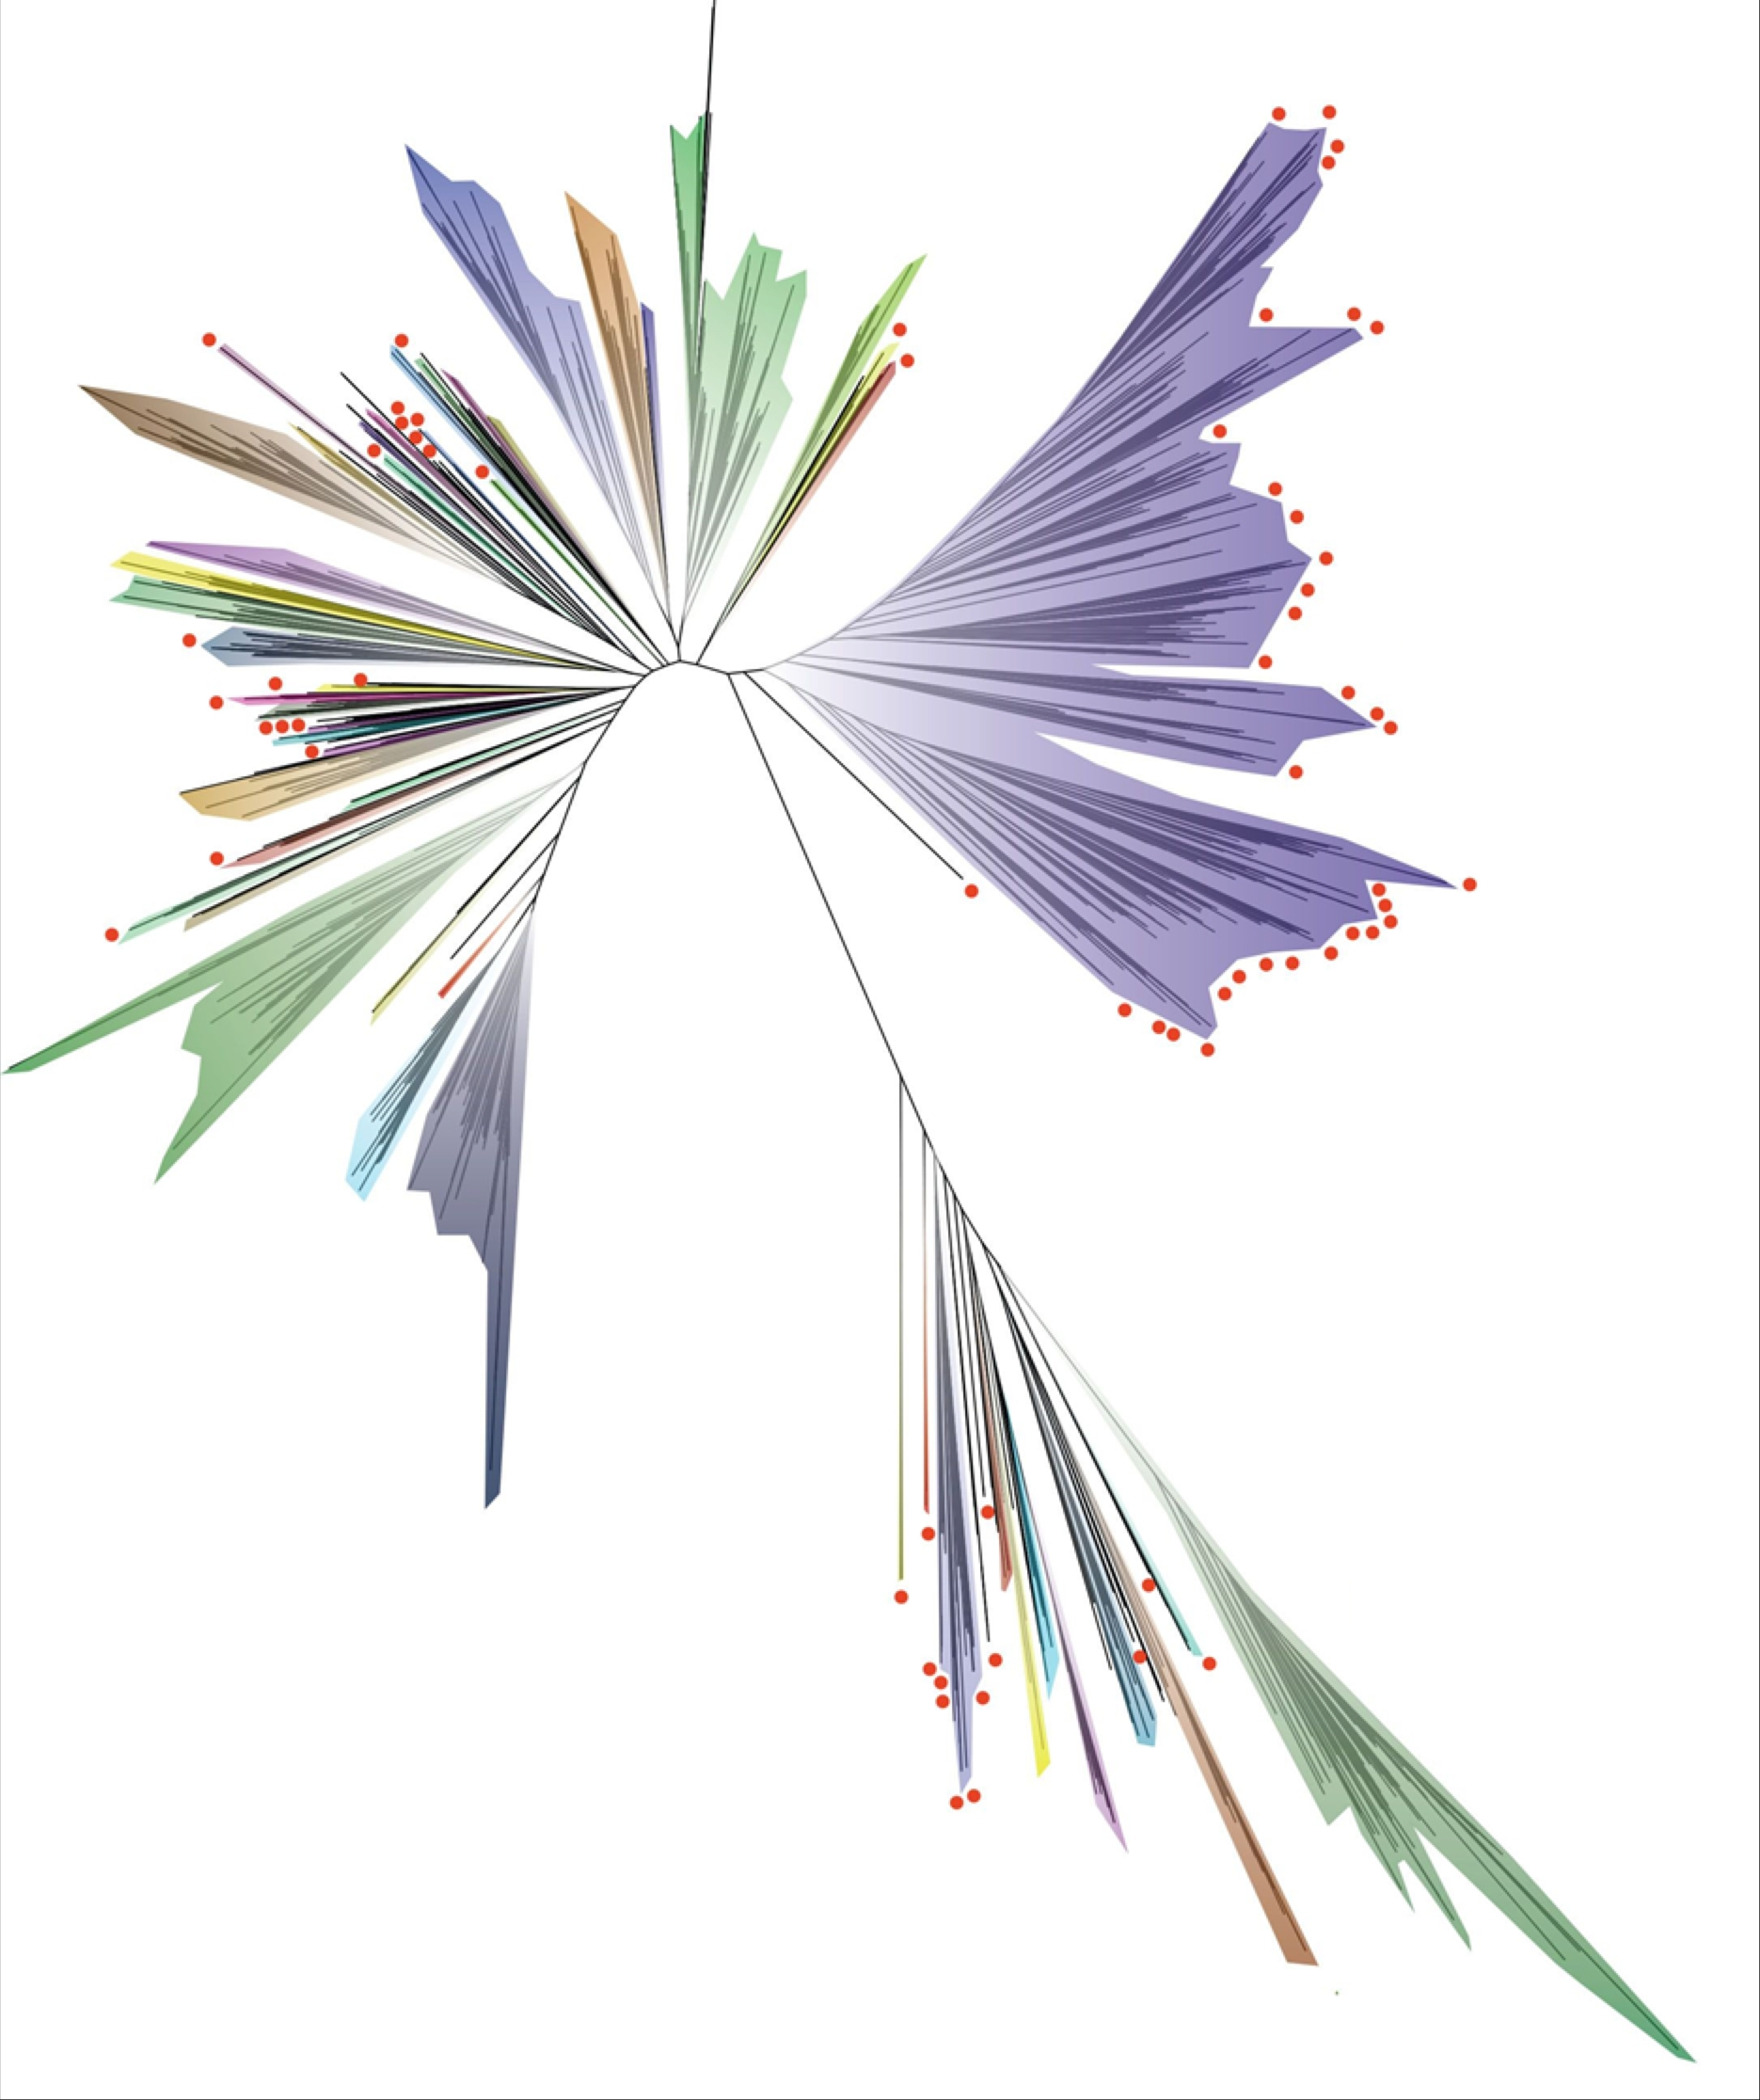
\includegraphics[width=0.9\textwidth]{TOL4}
\end{figure}

\begin{figure}[H]
	\caption{Unrooted phylogeny arises because mutation process is reversible in our models}\label{fig:unrooted:phylogeny}
	\begin{subfigure}[b]{0.45\textwidth}
		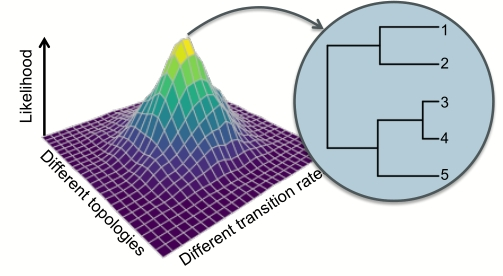
\includegraphics[width=\textwidth]{InferringPastHard1}
	\end{subfigure}
	\begin{subfigure}[b]{0.45\textwidth}
		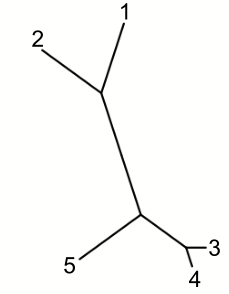
\includegraphics[width=\textwidth]{InferringPastHard2}
	\end{subfigure}
\end{figure}

The best method for finding a root is to use an \gls{gls:outgroup}--Figure \ref{fig:bird:outgroup}--which then gives a temporal direction to the tree: the tree flows away from the hypothetical common ancestor. But the Tree of [all] Life, by definition, has no outgroup!

\begin{figure}[H]
	\caption{Using a Bird as an Outgroup for the Tree of Mammals}\label{fig:bird:outgroup}
	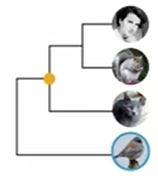
\includegraphics[width=0.9\textwidth]{Outgroup}
\end{figure}

Another problem is that rate heterogeneity means that mutations are not clock like. Time in a phylogeny is measured in substitutions, not in years. Since the rate of mutation varies across lineages and across Earth's history, mutation events don't tell us the time on each branch. So species in the Banfield Tree of Life--Figure \ref{fig:banfield:tol}-- don't line up.
\begin{itemize}
	\item We may be able to assign times from the fossil record.
	\item In some cases we \textit{do} know the mutation rate and can use it like a clock.
\end{itemize}

Caveat: long branches overlap. \cite{philippe2005heterotachy},

 What genetic information goes back to LUCA? Ribosomal RNA and protein genes.
 
   \cite{quast2012silva}, \cite{sanderson2003r8s}, \cite{smit2007evolutionary}

\section{Macroscopic Theories in Biology}

Lecturer: Chris Kempes

\begin{itemize}
	\item Which aspects of extant life are general, and which are arbitrary?
	\item How much of what we see is peculiar to the trajectory of life on our own planet?
	\item How much would be true of life anywhere?
\end{itemize}

This matters not just for exobiology, but also for understanding early life and the origin of life in general.

In this course we have covered:
\begin{itemize}
	\item Laws of chemistry
	\item General processes of natural selection
	\item Laws of physics
	\item Laws of Life?
\end{itemize}

As an example of Laws of Life, Figure \ref{fig:allometric:scaling} shows the Relationship between peak postfeeding resting metabolic rate and body mass for mammals\cite{white2005allometric}--an approximate power law with an exponent of $\frac{3}{4}$. West, Brown and Enquist have shown how this law follows from the fractal vascular structure of mammals \cite{west1997general}. Optimize so it fills space and bring nutrients to all cells, taking into account hydrodynamics, then wh get the $\frac{3}{4}$ exponent. The same thing works for plants. So Body Plan + Constraints$\rightarrow$Law of Life.

\begin{figure}[H]
	\caption{Relationship between peak postfeeding resting metabolic rate and body mass.}\label{fig:allometric:scaling}
	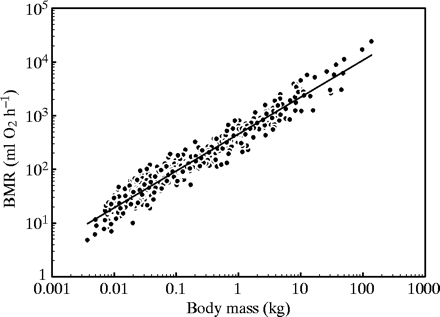
\includegraphics[width=0.9\textwidth]{WhiteSeymour}
\end{figure}


Example of a Fundamental Constraint: diffusion to a simple spherical cell drifting passively. Cell is living in a still fluid filled with nutrients, and we want to know how nutrients diffuse to cell. If we assume that cell uses all of nutrient, so concentration at surface is held at zero.

\begin{align*}
C(r) =& C_{\infty}\big(1 - \frac{r_C}{r}\big)\text{, where}\\
C_{\infty} =& \text{ concentartion at infinity}\\
C(r) =& \text{ concentration at distance r}\\
J(r) =& D\frac{\partial C}{\partial R} \text{ flux}\\
  =& D C_{\infty} \frac{r_c}{r^2}\\
U =& 4 \pi r_C^2 J(r_C) \text{ total uptake of nutrient}\\
=&4 \pi D C_{\infty} r_C 
\end{align*}

No rate process within the cell can use the nutrient more quickly than $U$, so all processes must scale with $r$ at this rate or more slowly. If process want to go faster than $U$, the fluid needs to be disturbed, or the cell needs to move.

Figure \ref{fig:BacterialPhysiology} shows the variation of component size with cell size\cite{kempes2016evolutionary}, and bounds the cell size: at the large end and small end the cell runs out of space for components.

\begin{figure}[H]
	\caption{BacterialPhysiology}\label{fig:BacterialPhysiology}
	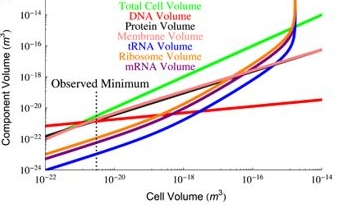
\includegraphics[width=0.9\textwidth]{BacterialPhysiology}
\end{figure}

We could see how the fundamental physiological constraint change for other conceivable forms of life.

See also \cite{kempes2011predicting}.

\section{Selection}

Lecturer: Michael Lachmann

''A naturalist, reflecting on the mutual affinities of organic beings, on their embryological relations, their geographical distribution, geological succession, and other such facts, might come to the conclusion that each species had not been independently created, but had descended, like varieties, from other  species''--Charles Darwin\cite{darwin1859origin}.

Darwin\cite{darwin1859origin} presented a phylogenetic Tree--\ref{fig:TOL:Darwin}. A modern view, Figure \ref{fig:TOL:Modern} is more like a web.

\begin{figure}[H]
	\caption{Two views of the Tree of Life}
	\begin{subfigure}[b]{0.45\textwidth}
		\caption{After Darwin}\label{fig:TOL:Darwin}
		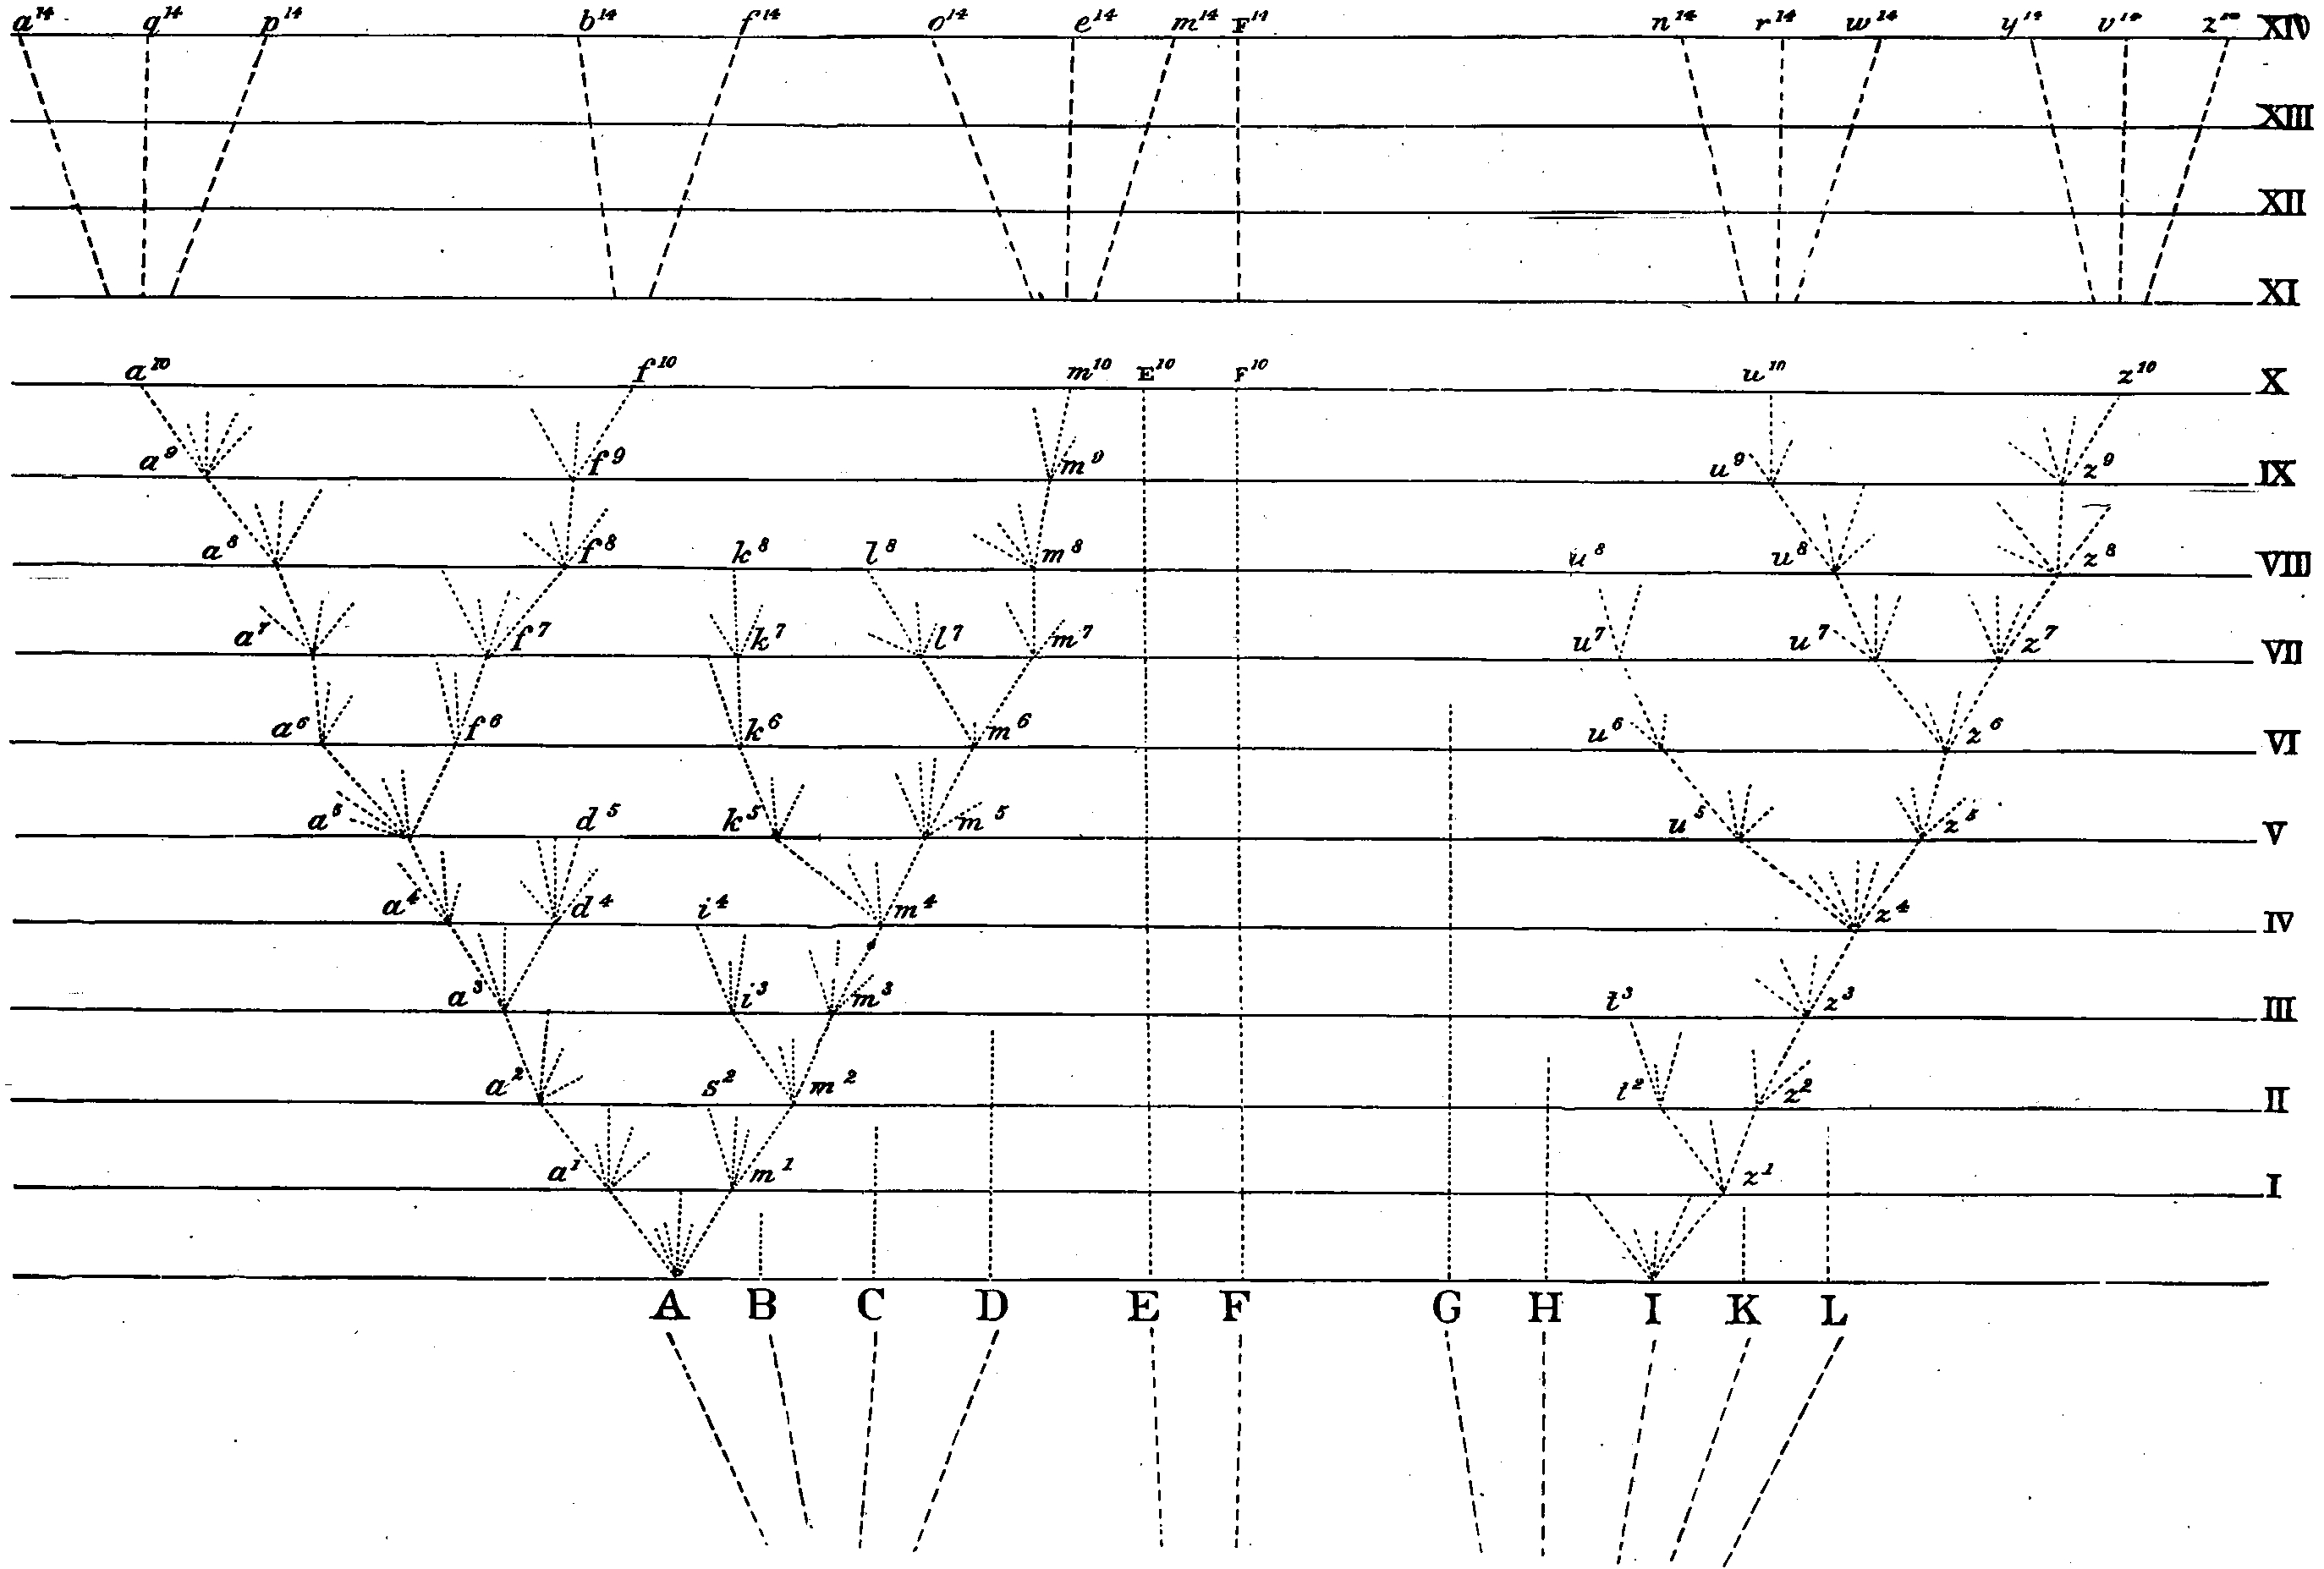
\includegraphics[width=\textwidth]{TOL_Darwin}
	\end{subfigure}
	\begin{subfigure}[b]{0.45\textwidth}
		\caption{Modern TOL}\label{fig:TOL:Modern}
		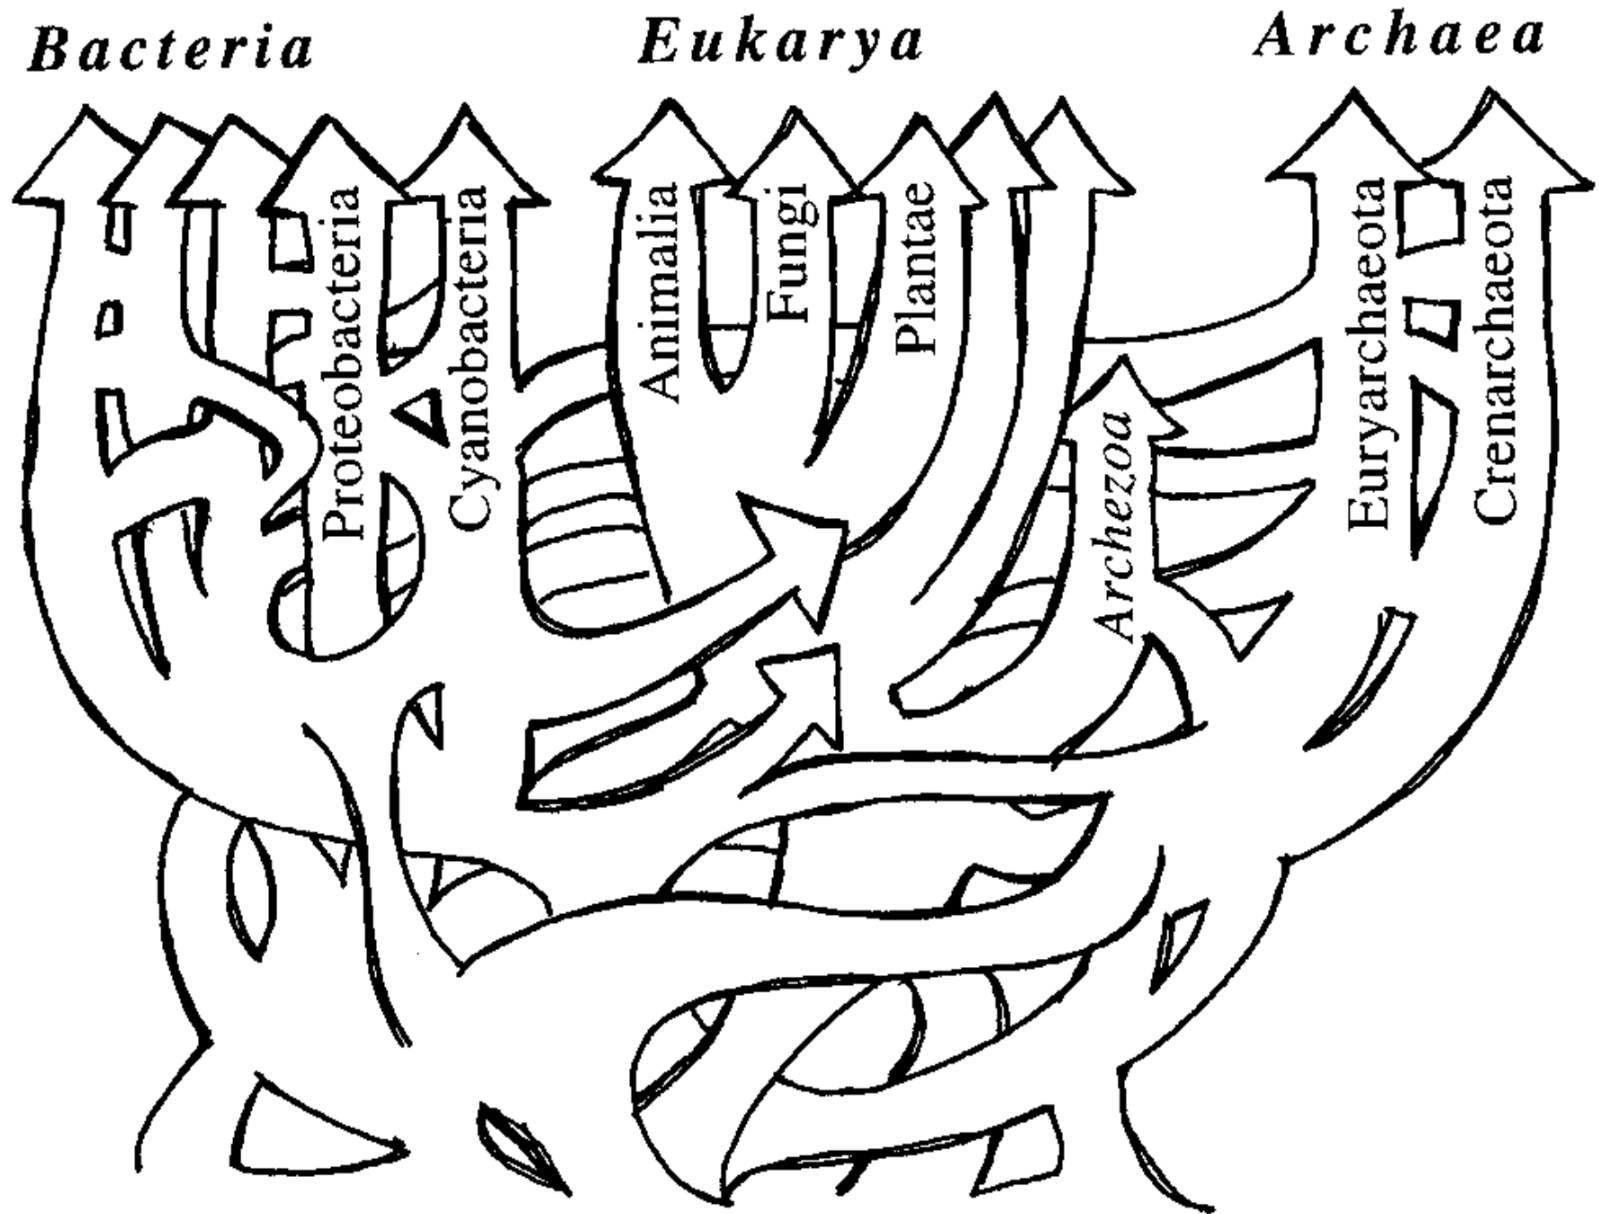
\includegraphics[width=\textwidth]{TOL-5-6}
	\end{subfigure}
\end{figure}

''Nevertheless, such a conclusion, even if well founded, would be unsatisfactory, until it could be shown how the innumerable species inhabiting this world have been modified, so as to acquire that perfection of structure and coadaptation which most justly excites our admiration''--\textit{ibid}.

How species acquire that perfection of structure:
\begin{itemize}
	\item Variation
	\item Inheritance
	\item Selection
\end{itemize}

\gls{gls:price:equation}--(\ref{eq:price:equation})

\begin{align*}
\Delta Z =& \frac{Cov(Z,W) + E(W \Delta Z)}{W}\text{, where} \numberthis \label{eq:price:equation}\\
Z=& \text{ some property, e.g. colour,}\\
W=& \text{ survival.}\\
 & \textit{Rearranging, }\\
W \Delta Z =& \underbrace{Cov(Z,W)}_\text{selection} + \underbrace{E(W \Delta Z)}_\text{transformation}
\end{align*}

How species acquire that perfection of structure? Because traits increase in value if they help individuals who have them survive, compared to those they don't.


\section{Artificial Life Theory}

Lecturer: Sara Imari Walker

Figure \ref{fig:PhysicsvsBiology} compares the evolution of a physical system with a biological system. Even the laws evolve in biology. Also biological systems involve homeostasis.
\begin{figure}[H]
	\caption{Physics: fixed law of evolution to final State, vs. Biology}\label{fig:PhysicsvsBiology}
	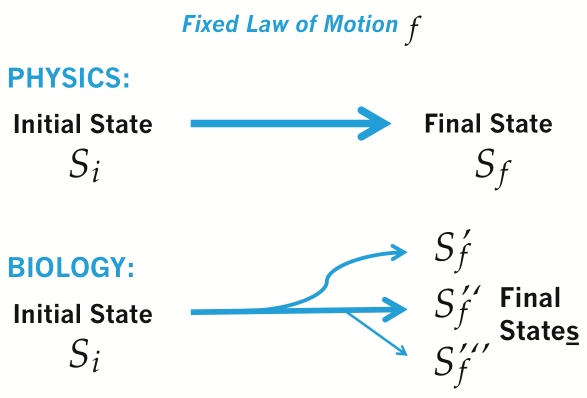
\includegraphics[width=0.9\textwidth]{PhysicsvsBiology}
\end{figure}

Von Neumann's work on self reproducing automata \cite{neumann1966theory}  \cite{neumann1958computer} is analogous to  the architecture of a modern cell--Figure \ref{fig:VonNeumann}. Note the instructional Tape in Figure  \ref{fig:VonNeumann1}--a small part of a larger biological algorithm. Note also that Von Neumann's work on cellular automata largely preceded our understanding of the translation from DNA to protein.



\begin{figure}[H]
	\caption{Von Neumann's work on self reproducing automata is analogous to the architecture of a modern cell}\label{fig:VonNeumann}
	\begin{subfigure}[b]{0.45\textwidth}
		\caption{The ribosome + assisting biomolecules
			act like a Universal Constructor}\label{fig:VonNeumann1}
		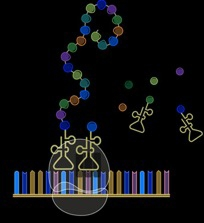
\includegraphics[width=\textwidth]{VonNeumann1}
	\end{subfigure}
	\begin{subfigure}[b]{0.45\textwidth}
		\caption{Supervisory Unit}\label{fig:VonNeumann2}
		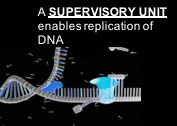
\includegraphics[width=\textwidth]{VonNeumann2}
	\end{subfigure}
\end{figure}

“physical” universality: the ability to implement any transformation whatsoever on any finite region \cite{janzing2010there}, \cite{schaeffer2014physicallyuniversal}

Are the ’laws of life’  the laws of information?
% end of text 

% glossary
\printglossaries

% bibliography go here
 
\bibliographystyle{unsrt}
\addcontentsline{toc}{section}{Bibliography}
\bibliography{origins}

\end{document}
